\documentclass[a4paper,12pt]{article}
\usepackage{ctex}
\usepackage{enumerate}
\usepackage{times}
\usepackage{multirow}
\usepackage{graphicx}
\usepackage{caption}
\usepackage{listings}
\usepackage{mathptmx}
\usepackage{amsmath}
\usepackage{amsfonts}
\usepackage[top=2cm, bottom=2cm, left=2cm, right=2cm]{geometry}

\usepackage{color}
\usepackage{alltt}
\usepackage[T1]{fontenc}

% highlight theme: XCode IDE
\newcommand{\hlstd}[1]{\textcolor[rgb]{0,0,0}{#1}}
\newcommand{\hlnum}[1]{\textcolor[rgb]{0.14,0,1}{#1}}
\newcommand{\hlesc}[1]{\textcolor[rgb]{0,0,0}{#1}}
\newcommand{\hlstr}[1]{\textcolor[rgb]{0.75,0,0}{#1}}
\newcommand{\hlpps}[1]{\textcolor[rgb]{0.45,0.22,0.06}{#1}}
\newcommand{\hlslc}[1]{\textcolor[rgb]{0,0.5,0.11}{#1}}
\newcommand{\hlcom}[1]{\textcolor[rgb]{0,0.5,0.11}{#1}}
\newcommand{\hlppc}[1]{\textcolor[rgb]{0.45,0.22,0.06}{#1}}
\newcommand{\hlopt}[1]{\textcolor[rgb]{0,0,0}{#1}}
\newcommand{\hlipl}[1]{\textcolor[rgb]{0,0,0}{#1}}
\newcommand{\hllin}[1]{\textcolor[rgb]{0.5,0.5,0.5}{#1}}
\newcommand{\hlkwa}[1]{\textcolor[rgb]{0.56,0,0.33}{#1}}
\newcommand{\hlkwb}[1]{\textcolor[rgb]{0.56,0,0.33}{#1}}
\newcommand{\hlkwc}[1]{\textcolor[rgb]{0.56,0,0.33}{#1}}
\newcommand{\hlkwd}[1]{\textcolor[rgb]{0,0,0}{#1}}

\begin{document}
  \title{����~1-3~��ҵ}
  \author{��������ۿԴ \and ѧ�ţ�161240004}
  \date{}
  \maketitle

  \section{[UD] Problem 6.12}
    Not always. Let $x=1$ and $y=-2$, since $x$ and $y$ are both nonzero, they are in $S$. However, $x~\#~y=x+y+1=1-2+1=0$ is zero, which means $x~\#~y$ is not in $S$.

  \section{[UD] Problem 6.14}
  \begin{enumerate}[(a)]
    \item Let $a=1$, $b=0$, $c=-4$, where $a, b, c$ are all integers with $a$ is nonzero. When $x=2$, the equality $ax^2+bx+c=x^2-4=0$ holds, therefore $2 \in A$. \hfill $\square$
    \item Let $a=1$, $b=0$, $c=-2$, where $a, b, c$ are all integers with $a$ is nonzero. When $x=\sqrt{2}$, we have $x^2-2=0$, so $\sqrt{2} \in A$. \hfill $\square$
    \item $\sqrt[3]2$.
    \item Let $p=a$, $q=b$, $r=c$. When $a, b, c$ are integers with at least one of them is nonzero, $p, q, r$ are rational numbers with at least one of them is nonzero. For every real number $x$, if $ax^2+bx+c=0$, then $px^2+qx+c=0$, so we have $A \subseteq B$. \\
        By the definition of rational numbers, there exists integers $m_p, n_p, m_q, n_q, m_r, n_r$ with $n_p, n_q, n_r \neq 0$ such that $p=\dfrac{m_p}{n_p}$, $q=\dfrac{m_q}{n_q}$ and $r=\dfrac{m_r}{n_r}$. Since at least one of $p, q, r$ is nonzero, at least one of $m_p, m_q, m_r$ is nonzero. Let $a=p n_p n_q n_r=m_p n_q n_r$, $b=q n_p n_q n_r=m_q n_p n_r$, $c=r n_p n_q n_r=m_r n_p n_q$, so $a, b, c$ are all integers and with at least one of them is nonzero. For every real number $x$, if $px^2+qx+r=0$, then $n_p n_q n_r(px^2+qx+r)=ax^2+bx+c=0$, so we have $B \subseteq A$. \\
        By the definition of equality of sets, we get $A=B$. \hfill $\square$
    \item By the definition of rational numbers, for every number $x \in \mathbb{Q}$, there exists two integers $m, n$ with $n \neq 0$ such that $x=\dfrac{m}{n}$. Let $a=0$, $b=n$, $c=-m$ with $c$ is nonzero, and we have $ax^2+bx+c=0$, so we get $\mathbb{Q} \subseteq A$. \hfill $\square$
  \end{enumerate}

  \section{[UD] Problem 6.15}
  \begin{enumerate}[(a)]
    \item $A$ is the graph of the inequality $y \neq 0$ with respect to $x$ and $y$. In other words, $A$ is a collection of points in a plane whose y-coordinate are nonzero.
    \item Since $(x,y)$, $(z,w)$ are elements of $A$, we have $y \neq 0$ and $w \neq 0$. Thus, $wy \neq 0$, which means $(xw+zy, wy)$ is again an object in $A$. \hfill $\square$
    \item $(a,b) \diamond (x,y)=(ay+bx,by)=(x,y)$ holds for every $(x,y)$ in $A$. Compare the coefficients of $x,y$, we get $a=0$ and $b=1$, so the element is $(0,1)$.
    \item For every element $(a,b)$ in $A$, if we regard $a$ as the numerator, and $b$ as the denominator, we can find that this ``new'' addition shows the addition of two fractions:
        $$\frac{x}{y}+\frac{z}{w}=\frac{xw+zy}{wy}.$$
  \end{enumerate}

  \section{[UD] Problem 6.18}
    No. Consider $\left(\dfrac{\sqrt{2}}{2},\dfrac{\sqrt{2}}{2}\right)$, we have $\left(\dfrac{\sqrt{2}}{2}\right) ^2 + \left(\dfrac{\sqrt{2}}{2}\right) ^2=1 \leq 1$ and $\left|\dfrac{\sqrt{2}}{2}\right|+\left|\dfrac{\sqrt{2}}{2}\right|=\sqrt{2}>1$, so $\left(\dfrac{\sqrt{2}}{2},\dfrac{\sqrt{2}}{2}\right)$ is an element of the first set and it is not an element of the second set. Therefore the second set is not a subset of the first set, and thus the two sets are not equal. \hfill $\square$

  \section{[UD] Problem 17.11}
  \begin{enumerate}[(a)]
    \item Take $m=0$ and $n=1$, we have $g(1)=g(0)g(1)$. Cancel the positive real number $g(1)=a$ on both sides, we get $g(0)=0$. \hfill $\square$
    \item Let $P(n)$ denote that $g(n)=a^n$. For the base step, we have to check $g(1)=1$, this is obviously true because this is one of the properties of $g$. \par
        For the induction step, assume that $P(n)$ holds for a positive integer $n$. That is $g(n)=a^n$. Apply the second property of $g$, we get $g(n+1)=g(n)g(1)=a^n \times a=a^{n+1}$. Thus, $P(n+1)$ holds. \par
        By mathematical induction, we conclude that $g(n)=a^n$ for all $n \in \mathbb{N}$. \hfill $\square$
  \end{enumerate}

  \section{[UD] Problem 17.13}
    Let $P(n)$ denote that $p(c)=0$ implies $c=0$ for every polynomial $p(x)$ of order $n$ satisfies the conditions in the nontheorem. The implication $P(1) \rightarrow P(2)$ doesn't hold. When $n=2$, $p(c)$ has only two factors, so if we remove one factor to form $q(x)$, $q(x)$ must be a 1-order polynomial and $q(c)$ doesn't have the factor $ac(a_1c+b_1)$.

  \section{[UD] Problem 17.14}
  Let $P(n)$ denote that ``$Q(1),\dots,Q(n)$'' are all true. For the base step, let $n=1$. $P(1)$ is certainly true because $Q(1)$ is true. \par
  For the induction step, assume that $P(n)$ is true where $n$ is a positive integer, i.e. $Q(1),\dots,Q(n)$ are all true. By supposition (ii), we have that $Q(n+1)$ is true. $Q(n+1)$, along with $Q(1),\dots,Q(n)$ are all true, thus $P(n+1)$ is true. \par
  By mathematical induction, we conclude that $P(n)$ holds for all positive integers $n$. Therefore, $Q(n)$ holds for all positive integers $n$.  \hfill $\square$

  \section{[UD] Problem 17.16}
  For the base step, we have to prove that the sum of all the interior angles of a triangle is $180^\circ$. Let $\triangle ABC$ be a triangle. Draw line $l$ through point $A$ and parallel to $BC$. By the property of parallel lines, we have that $\angle 1 = \angle C$, $\angle 3 = \angle B$, so the sum of all the interior angles of a triangle is $\angle A + \angle B + \angle C = \angle 2 + \angle 3 + \angle 1 = 180^\circ$.
  \begin{figure}[htbp]
    \centering
    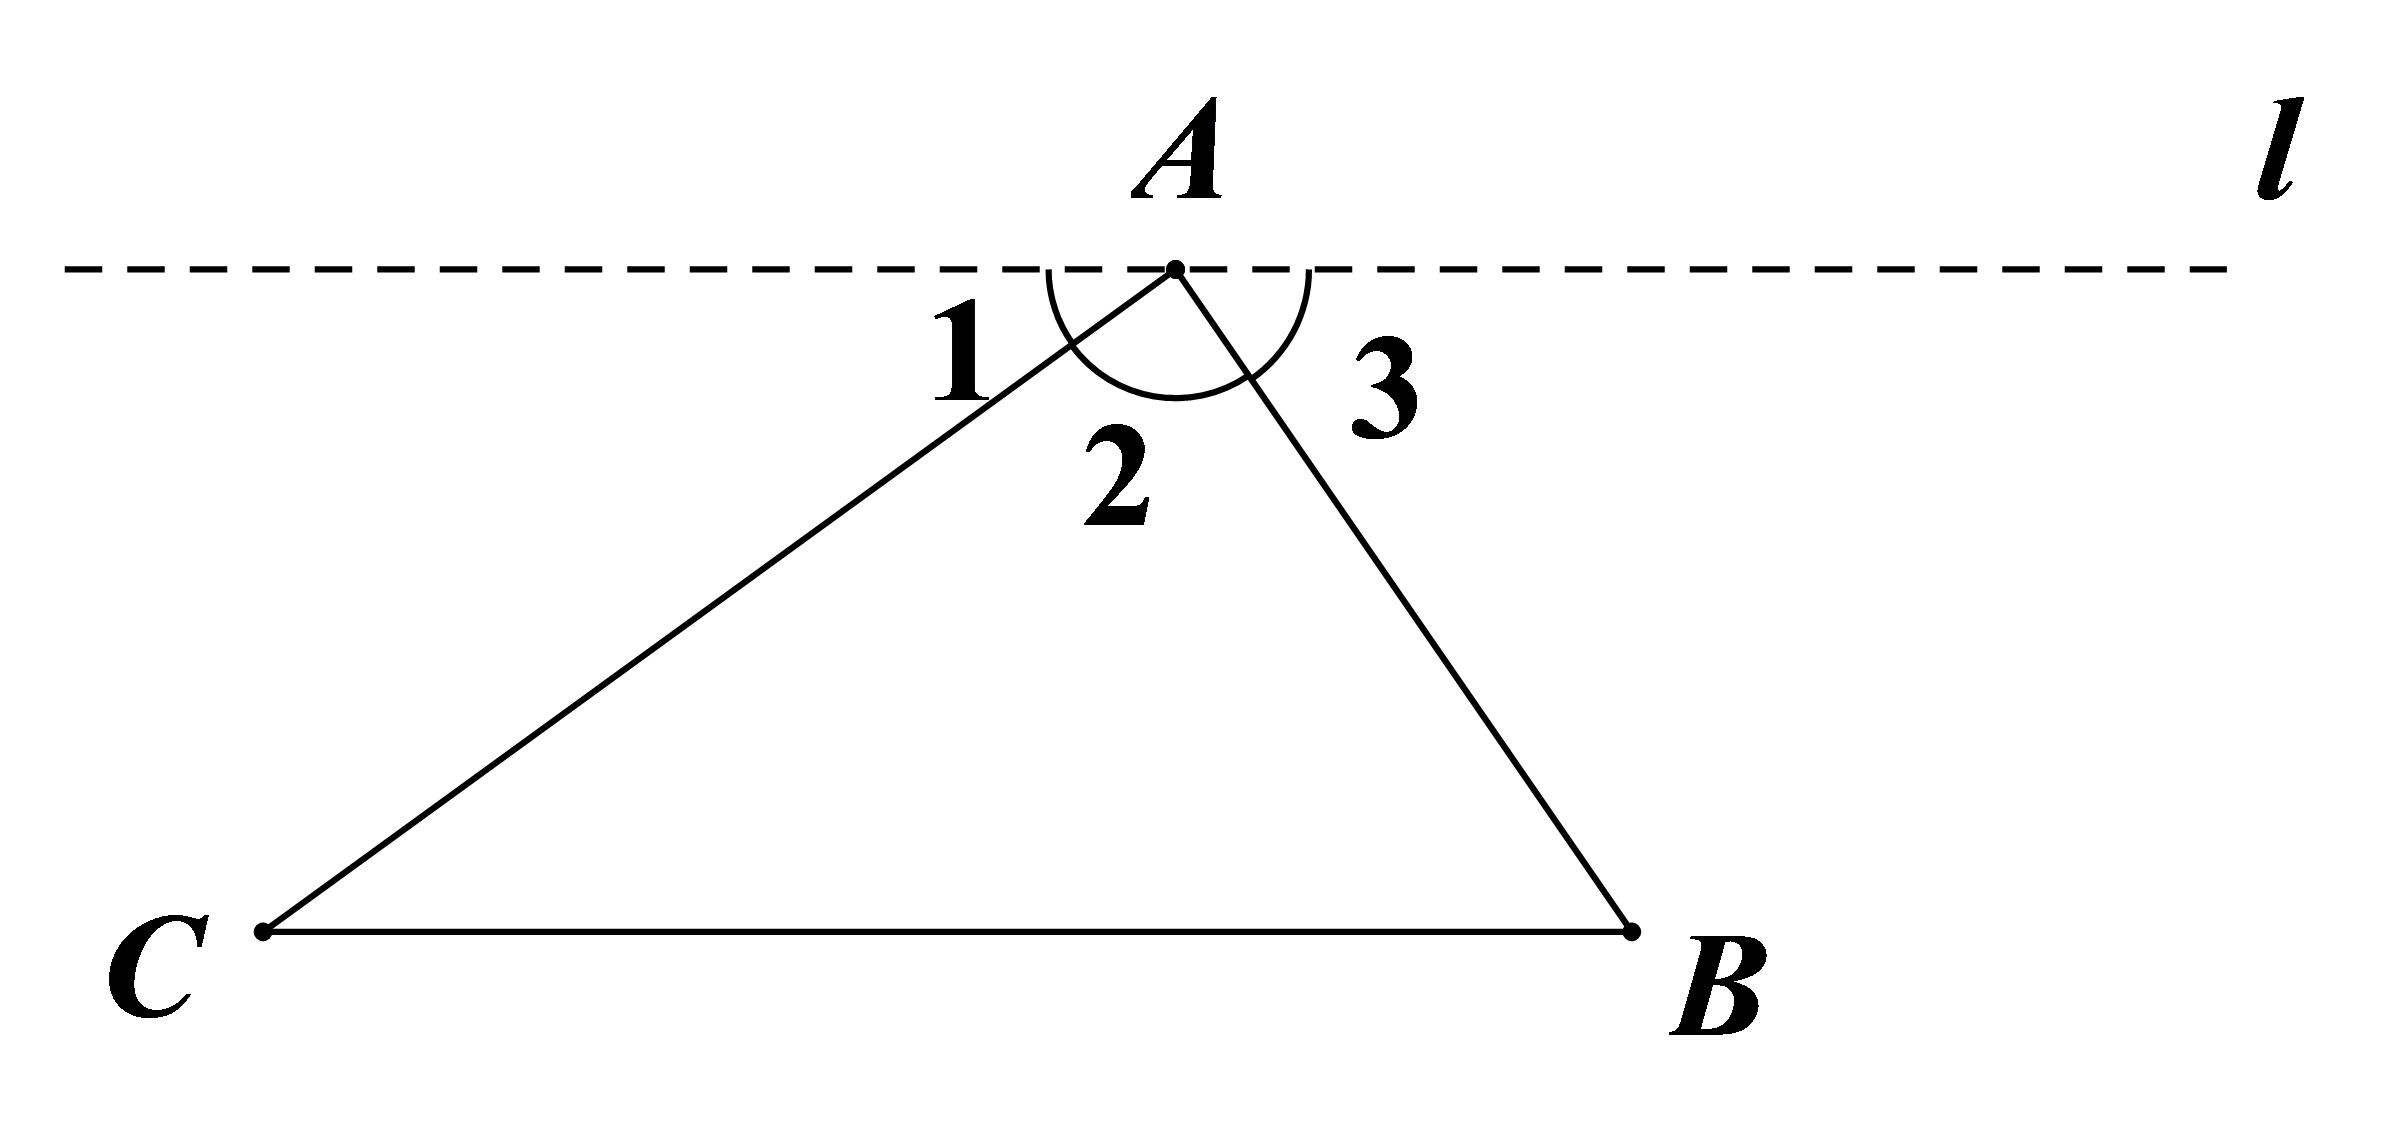
\includegraphics[width=6cm]{figures/fig1.png} \\
    \caption*{Figure 1: the sum of all the interior angles of a triangle is $180^\circ$}
  \end{figure} \par
  For the induction step, assume that the sum of all the interior angles of a convex polygon with $n$ $(n \geq 3, n \in \mathbb{N})$ vertices is $(n-2)180^\circ$. Let $A_1 A_2 \cdots A_{n-1} A_n A_{n+1}$ be a convex polygon with $n+1$ vertices. Draw a line through $A_1 A_n$, then $A_1 A_n A_{n+1}$ is a triangle, of which the sum of all the interior angles is $180^\circ$, and a convex polygon with $n$ vertices, of which the sum of all the interior angles is $(n-2)180^\circ$ by induction hypothesis. So the sum of all the interior angles of $A_1 A_2 \cdots A_{n-1} A_n A_{n+1}$ is $\angle A_1 + \angle A_2 + \cdots + \angle A_{n+1} = (\angle A_{n+1} + \angle A_{n+1} A_n A_1 + \angle A_{n+1} A_1 A_n) + (\angle A_{n-1} A_n A_1+ \angle A_n A_1 A_2 + \angle A_1 + \cdots + \angle A_{n-1}) = 180^\circ + (n-2)180^\circ = [(n+1)-2]180^\circ$.
  \begin{figure}[htbp]
    \centering
    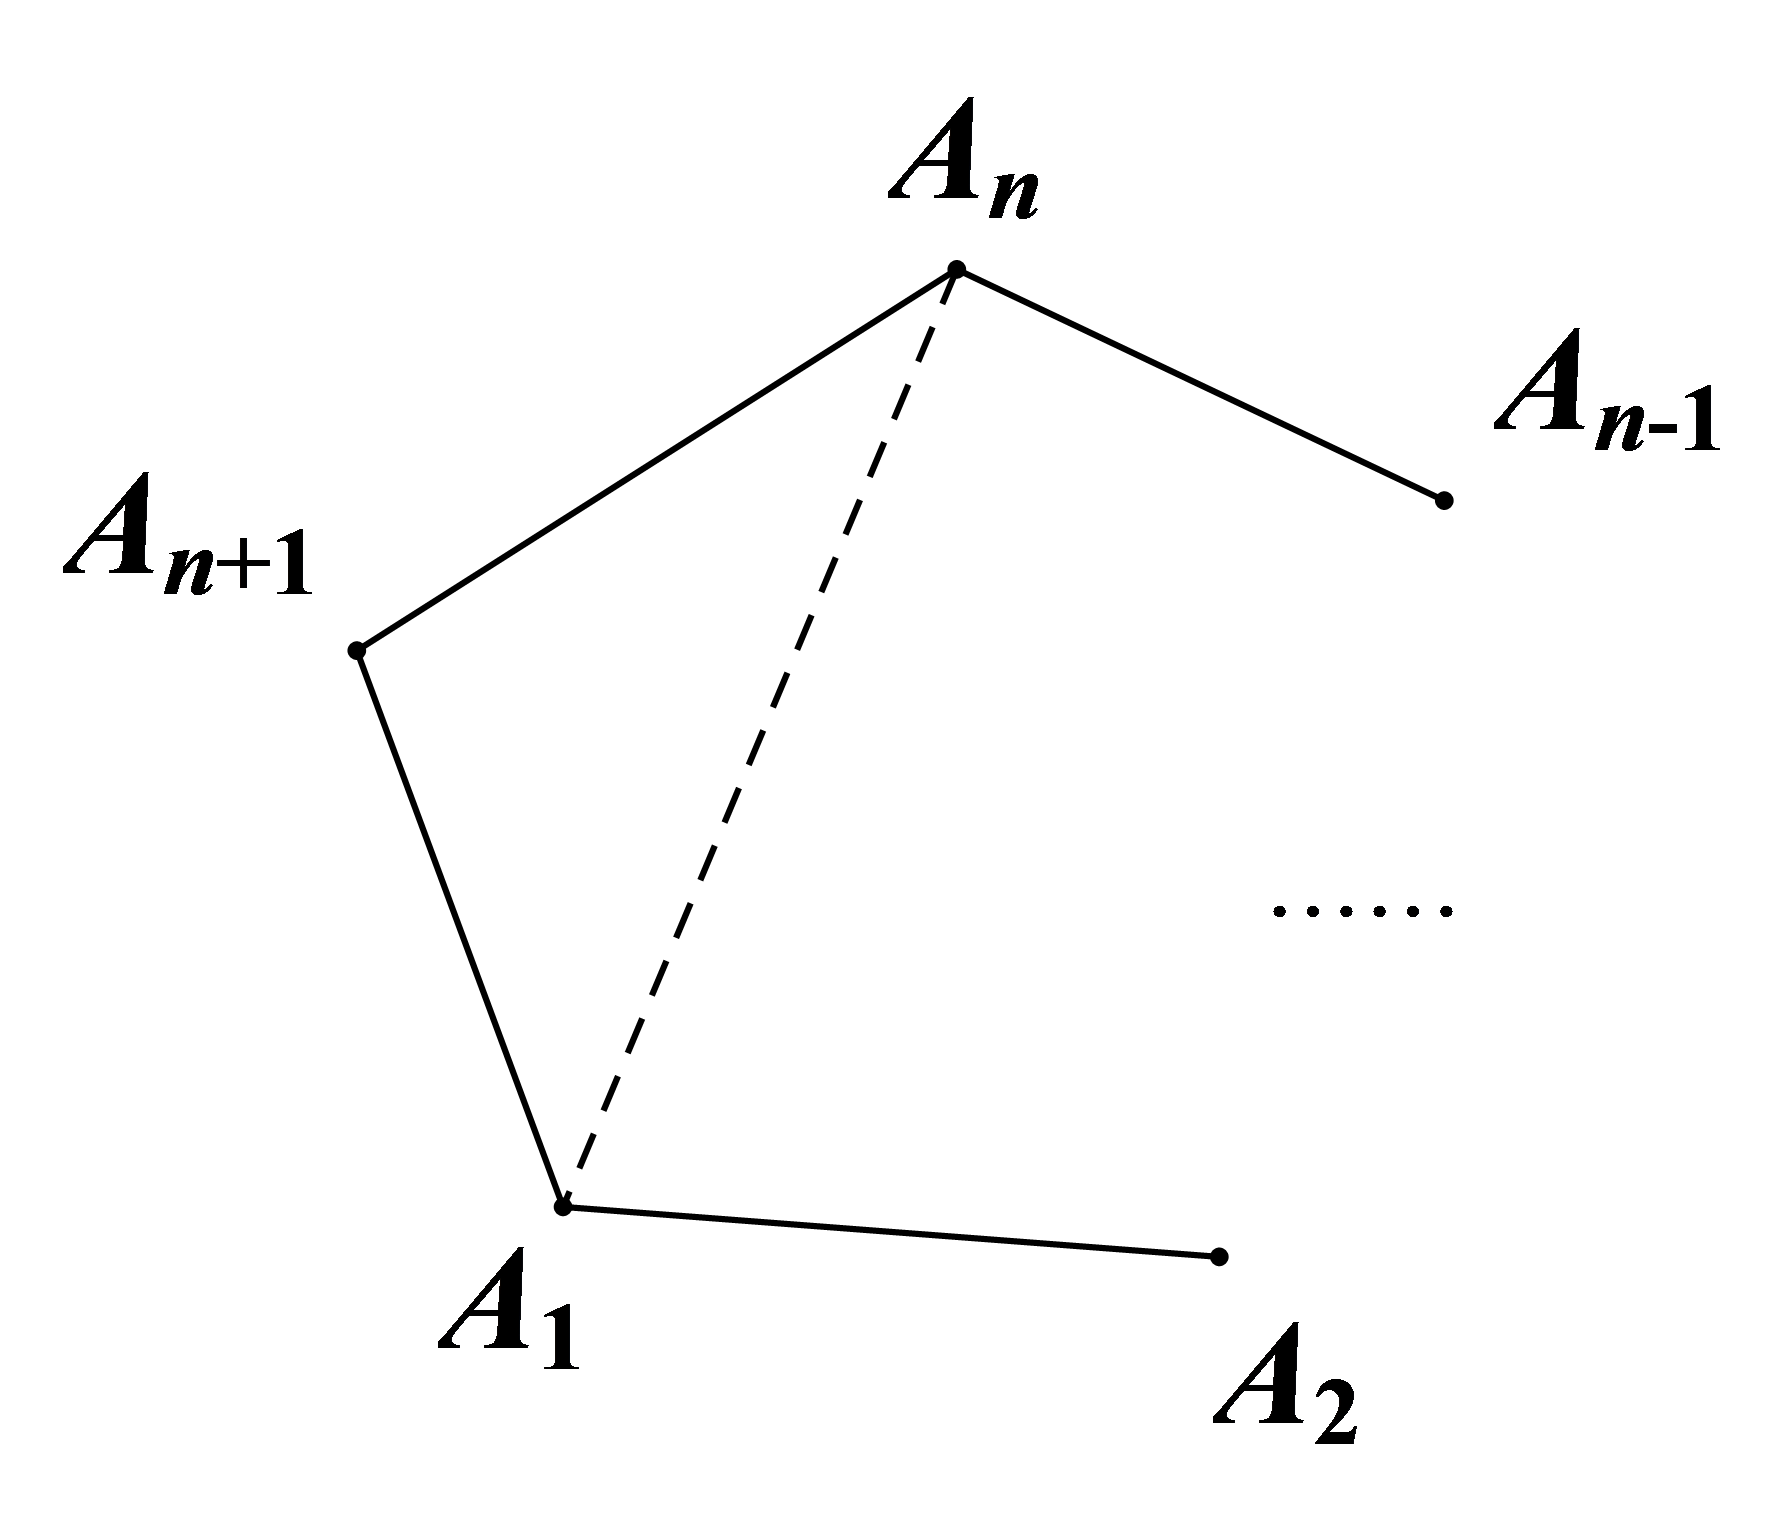
\includegraphics[width=6cm]{figures/fig2.png} \\
    \caption*{Figure 2: a convex polygon with $n+1$ vertices}
  \end{figure} \par
  By mathematical induction, we conclude that for all integers $n$ where $n \geq 3$, the sum of all the interior angles of a convex polygon with $n$ vertices is $(n-2)180^\circ$. \hfill $\square$

  \section{[UD] Problem 17.18}
  \begin{enumerate}[(a)]
    \item $T_n=\dfrac{n(n+1)}{2}$. \par
    Proof: The validity of the base step is obvious. Now assume that $T_n=\dfrac{n(n+1)}{2}$. We can find that $T_{n+1}=T_n + (n+1)$, so $T_{n+1}=\dfrac{n(n+1)}{2} + (n+1) = \dfrac{n(n+1)+2n+2}{2} = \dfrac{(n+1)(n+2)}{2}$. \par
    By mathematical induction, we conclude that $T_n=\dfrac{n(n+1)}{2}$ holds for all positive integers $n$. \hfill $\square$
    \item
  \end{enumerate}

  \section{[UD] Problem 17.19}
  \begin{enumerate}[(a)]
    \item $5!=120$, $\begin{pmatrix}8\\3\end{pmatrix}=56$, $\begin{pmatrix}8\\5\end{pmatrix}=56$, $\begin{pmatrix}5\\2\end{pmatrix}=10$, $\begin{pmatrix}5\\3\end{pmatrix}=10$ , $\begin{pmatrix}7\\0\end{pmatrix}=1$, $\begin{pmatrix}7\\7\end{pmatrix}=1$.
    \item $(m+1)^2$ equally spaced dots form a square with sides built of $m+1$ equally spaced dots. Divide these dots into four parts as the picture shows. There are $m^2$ dots in the upper-left part, $m$ dots in the upper-right part, $m$ dots in the lower-left part and one dot in the lower-right part. Thus  $(m+1)^2=m^2+2m+1$.
    \item By the definition of binomial coefficient, we have
    \begin{align*}
        \begin{pmatrix}n\\k-1\end{pmatrix}+\begin{pmatrix}n\\k\end{pmatrix}&=
        \frac{n!}{(k-1)!(n-k+1)!}+\frac{n!}{k!(n-k)!}\\
        &=\frac{n!k}{k!(n-k+1)!}+\frac{n!(n-k+1)}{k!(n-k+1)!}\\
        &=\frac{(n+1)!}{k!(n-k+1)!} \\
        &=\frac{(n+1)!}{k!(n-k+1)!} \\
        &=\begin{pmatrix}n+1\\k\end{pmatrix} & \square
    \end{align*}
    \item We use mathematical induction. For the base step, we have to check that $a+b=\begin{pmatrix}1\\0\end{pmatrix}b+\begin{pmatrix}1\\1\end{pmatrix}a$, which is certainly true. \par
        For the induction step, assume that
        $$(a+b)^n=\sum\limits_{k=0}^n \begin{pmatrix}n\\k\end{pmatrix} a^{k} b^{n-k}$$ holds for every $a$ and $b$. Then,
        \begin{align*}
          (a+b)^{n+1}&=(a+b)(a+b)^n \\
          &= (a+b) \sum\limits_{k=0}^n \begin{pmatrix} n\\k \end{pmatrix} a^{k} b^{n-k} \\
          &= \sum\limits_{k=0}^n \begin{pmatrix} n\\k \end{pmatrix} a^{k+1} b^{n-k}+\sum\limits_{k=0}^n \begin{pmatrix} n\\k \end{pmatrix} a^{k} b^{n-k+1} \\
          &= \sum\limits_{k=1}^{n+1} \begin{pmatrix} n\\k-1 \end{pmatrix} a^{k} b^{n-k+1}+\sum\limits_{k=0}^n \begin{pmatrix} n\\k \end{pmatrix} a^{k} b^{n-k+1} \\
          &= a^{n+1}+b^{n+1}+\sum\limits_{k=1}^{n} \left[\begin{pmatrix} n\\k-1 \end{pmatrix}+\begin{pmatrix} n\\k \end{pmatrix}\right] a^{k} b^{n-k+1}\\
          &= a^{n+1}+b^{n+1}+\sum\limits_{k=1}^{n} \begin{pmatrix} n+1\\k \end{pmatrix} a^{k} b^{n-k+1}\\
          &= \sum\limits_{k=0}^{n+1} \begin{pmatrix} n+1\\k \end{pmatrix} a^{k} b^{n-k+1}
        \end{align*}
        By mathematical induction, we conclude that $\displaystyle (a+b)^n=\sum\limits_{k=0}^n \begin{pmatrix}n\\k\end{pmatrix} a^{k} b^{n-k}$. \hfill $\square$
    \item Take $a=-1, b=1$ and apply binomial theorem, the left side is identically zero, the right side is $\displaystyle
        \sum \limits _{k=0}^n\begin{pmatrix}n\\k\end{pmatrix}(-1)^k$, so $\displaystyle \sum \limits _{k=0}^n\begin{pmatrix}n\\k\end{pmatrix}(-1)^k=0$. \hfill $\square$
  \end{enumerate}

  \section{[ES] Problem 24.4}
    Divide the square into four identical small squares as Figure 3 shows. Each small square includes its border. By the Pigeonhole Principle, there exists one small square who has at least two points. In one small square, the maximum of the distance of two points is $\sqrt{2}/2$, the length of the diagonal. So there always exist two points whose distance is at most $\sqrt{2}/2$. \hfill $\square$
  \begin{figure}[htbp]
    \centering
    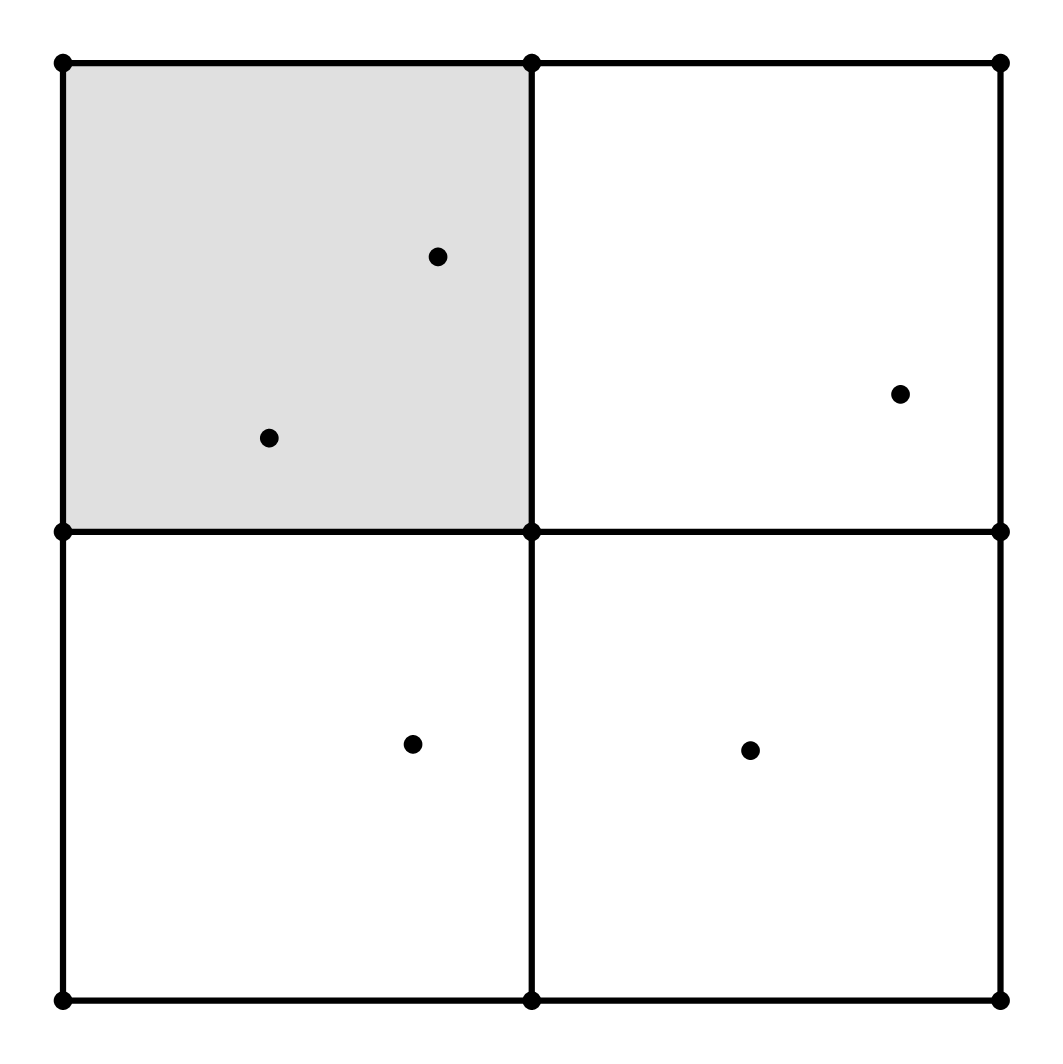
\includegraphics[width=5cm]{figures/fig3.png} \\
    \caption*{Figure 3: the square is divided into four small squares}
  \end{figure}

  \section{[ES] Problem 24.6}
    \paragraph{Proposition} Give nine distinct lattice points in three-dimensional space, at least one of the segments determined by these points has a lattice point as its midpoint.
    \paragraph{Proof} Classify the nine points into eight types by the parity of their coordinates:
      $$\begin{matrix}
        (even, even, even) &(even, even, odd) &(even, odd, even) &(even, odd, odd) \\
        (odd, even, even) &(odd, even, odd) &(odd, odd, even) &(odd, odd, odd)
      \end{matrix}$$
    By the Pigeonhole Principle, there exist two points who have the same parity. Let $(a, b, c)$ and $(d, e, f)$ be the two points, recall the midpoint formula, the coordinates of their midpoint are
    $$ \left(\frac{a+d}{2}, \frac{b+e}{2}, \frac{c+f}{2}\right).$$
    $\dfrac{a+d}{2}$ is an integer because $a$ and $d$ share the same parity. $\dfrac{b+e}{2}$ and $\dfrac{c+f}{2}$ are integers likewise. This proves that the midpoint is a lattice point. \hfill $\square$

  \section{[ES] Problem 24.8}

\newsavebox{\hlboxopenbrace}
\newsavebox{\hlboxclosebrace}
\newsavebox{\hlboxlessthan}
\newsavebox{\hlboxgreaterthan}
\newsavebox{\hlboxdollar}
\newsavebox{\hlboxunderscore}
\newsavebox{\hlboxand}
\newsavebox{\hlboxhash}
\newsavebox{\hlboxat}
\newsavebox{\hlboxbackslash}
\newsavebox{\hlboxpercent}
\newsavebox{\hlboxhat}
\setbox\hlboxopenbrace=\hbox{\verb.{.}
\setbox\hlboxclosebrace=\hbox{\verb.}.}
\setbox\hlboxlessthan=\hbox{\verb.<.}
\setbox\hlboxgreaterthan=\hbox{\verb.>.}
\setbox\hlboxdollar=\hbox{\verb.$.}
\setbox\hlboxunderscore=\hbox{\verb._.}
\setbox\hlboxand=\hbox{\verb.&.}
\setbox\hlboxhash=\hbox{\verb.#.}
\setbox\hlboxat=\hbox{\verb.@.}
\setbox\hlboxbackslash=\hbox{\verb.\.}
\setbox\hlboxpercent=\hbox{\verb.\%.}
\setbox\hlboxhat=\hbox{\verb.^.}
\noindent\tt{
Language: C++\\
\hlstd{}\hlppc{\#include\ \usebox{\hlboxlessthan}iostream\usebox{\hlboxgreaterthan}}\hspace*{\fill}\\
\hlstd{}\hlppc{\#include\ \usebox{\hlboxlessthan}algorithm\usebox{\hlboxgreaterthan}}\hspace*{\fill}\\
\hlstd{}\hlkwa{using\ namespace\ }\hlstd{std}\hlopt{;}\hspace*{\fill}\\
\hlstd{}\hspace*{\fill}\\
\hlstd{}\hlkwb{int\ }\hlstd{arr}\hlopt{{[}}\hlstd{}\hlnum{1050}\hlstd{}\hlopt{{]};}\hspace*{\fill}\\
\hlstd{}\hlkwb{int\ }\hlstd{n\ }\hlopt{=\ }\hlstd{}\hlnum{0}\hlstd{}\hlopt{;}\hspace*{\fill}\\
\hlstd{}\hlkwb{int\ }\hlstd{s}\hlopt{{[}}\hlstd{}\hlnum{1050}\hlstd{}\hlopt{{]};}\hspace*{\fill}\\
\hlstd{}\hlkwb{int\ }\hlstd{top\ }\hlopt{=\ }\hlstd{}\hlnum{0}\hlstd{}\hlopt{;}\hspace*{\fill}\\
\hlstd{}\hspace*{\fill}\\
\hlstd{}\hlkwb{int\ }\hlstd{}\hlkwd{main}\hlstd{}\hlopt{()}\hspace*{\fill}\\
\hlstd{}\hlopt{\usebox{\hlboxopenbrace}}\hspace*{\fill}\\
\hlstd{}\hlstd{\ \ \ \ }\hlstd{}\hlkwb{int\ }\hlstd{ans}\hlopt{;}\hspace*{\fill}\\
\hlstd{}\hlstd{\ \ \ \ }\hlstd{}\hlkwb{int\ }\hlstd{temp}\hlopt{;}\hspace*{\fill}\\
\hlstd{}\hlstd{\ \ \ \ }\hlstd{}\hlkwa{while\ }\hlstd{}\hlopt{(}\hlstd{cin\ }\hlopt{\usebox{\hlboxgreaterthan}\usebox{\hlboxgreaterthan}\ }\hlstd{arr}\hlopt{{[}}\hlstd{n}\hlopt{{]})\ }\hlstd{n}\hlopt{++;}\hspace*{\fill}\\
\hlstd{}\hlstd{\ \ \ \ }\hlstd{}\hlkwa{for\ }\hlstd{}\hlopt{(}\hlstd{}\hlkwb{int\ }\hlstd{i\ }\hlopt{=\ }\hlstd{}\hlnum{0}\hlstd{}\hlopt{;\ }\hlstd{i\ }\hlopt{\usebox{\hlboxlessthan}\ }\hlstd{n}\hlopt{;\ }\hlstd{i}\hlopt{++)}\hspace*{\fill}\\
\hlstd{}\hlstd{\ \ \ \ }\hlstd{}\hlopt{\usebox{\hlboxopenbrace}}\hspace*{\fill}\\
\hlstd{}\hlstd{\ \ \ \ \ \ \ \ }\hlstd{temp\ }\hlopt{=\ }\hlstd{}\hlkwd{upper\textunderscore bound}\hlstd{}\hlopt{(}\hlstd{s}\hlopt{,\ }\hlstd{s\ }\hlopt{+\ }\hlstd{top}\hlopt{,\ }\hlstd{arr}\hlopt{{[}}\hlstd{i}\hlopt{{]})\ {-}\ }\hlstd{s}\hlopt{;}\hspace*{\fill}\\
\hlstd{}\hlstd{\ \ \ \ \ \ \ \ }\hlstd{s}\hlopt{{[}}\hlstd{temp}\hlopt{{]}\ =\ }\hlstd{arr}\hlopt{{[}}\hlstd{i}\hlopt{{]};}\hspace*{\fill}\\
\hlstd{}\hlstd{\ \ \ \ \ \ \ \ }\hlstd{top\ }\hlopt{=\ }\hlstd{}\hlkwd{max}\hlstd{}\hlopt{(}\hlstd{temp\ }\hlopt{+\ }\hlstd{}\hlnum{1}\hlstd{}\hlopt{,\ }\hlstd{top}\hlopt{);}\hspace*{\fill}\\
\hlstd{}\hlstd{\ \ \ \ }\hlstd{}\hlopt{\usebox{\hlboxclosebrace}}\hspace*{\fill}\\
\hlstd{}\hlstd{\ \ \ \ }\hlstd{ans\ }\hlopt{=\ }\hlstd{top}\hlopt{;}\hspace*{\fill}\\
\hlstd{}\hlstd{\ \ \ \ }\hlstd{top\ }\hlopt{=\ }\hlstd{}\hlnum{0}\hlstd{}\hlopt{;}\hspace*{\fill}\\
\hlstd{}\hlstd{\ \ \ \ }\hlstd{}\hlkwa{for\ }\hlstd{}\hlopt{(}\hlstd{}\hlkwb{int\ }\hlstd{i\ }\hlopt{=\ }\hlstd{}\hlnum{0}\hlstd{}\hlopt{;\ }\hlstd{i\ }\hlopt{\usebox{\hlboxlessthan}\ }\hlstd{n}\hlopt{;\ }\hlstd{i}\hlopt{++)}\hspace*{\fill}\\
\hlstd{}\hlstd{\ \ \ \ }\hlstd{}\hlopt{\usebox{\hlboxopenbrace}}\hspace*{\fill}\\
\hlstd{}\hlstd{\ \ \ \ \ \ \ \ }\hlstd{arr}\hlopt{{[}}\hlstd{i}\hlopt{{]}\ =\ {-}}\hlstd{arr}\hlopt{{[}}\hlstd{i}\hlopt{{]};}\hspace*{\fill}\\
\hlstd{}\hlstd{\ \ \ \ \ \ \ \ }\hlstd{temp\ }\hlopt{=\ }\hlstd{}\hlkwd{upper\textunderscore bound}\hlstd{}\hlopt{(}\hlstd{s}\hlopt{,\ }\hlstd{s\ }\hlopt{+\ }\hlstd{top}\hlopt{,\ }\hlstd{arr}\hlopt{{[}}\hlstd{i}\hlopt{{]})\ {-}\ }\hlstd{s}\hlopt{;}\hspace*{\fill}\\
\hlstd{}\hlstd{\ \ \ \ \ \ \ \ }\hlstd{s}\hlopt{{[}}\hlstd{temp}\hlopt{{]}\ =\ }\hlstd{arr}\hlopt{{[}}\hlstd{i}\hlopt{{]};}\hspace*{\fill}\\
\hlstd{}\hlstd{\ \ \ \ \ \ \ \ }\hlstd{top\ }\hlopt{=\ }\hlstd{}\hlkwd{max}\hlstd{}\hlopt{(}\hlstd{temp\ }\hlopt{+\ }\hlstd{}\hlnum{1}\hlstd{}\hlopt{,\ }\hlstd{top}\hlopt{);}\hspace*{\fill}\\
\hlstd{}\hlstd{\ \ \ \ }\hlstd{}\hlopt{\usebox{\hlboxclosebrace}}\hspace*{\fill}\\
\hlstd{}\hlstd{\ \ \ \ }\hlstd{cout\ }\hlopt{\usebox{\hlboxlessthan}\usebox{\hlboxlessthan}\ }\hlstd{}\hlkwd{max}\hlstd{}\hlopt{(}\hlstd{ans}\hlopt{,\ }\hlstd{top}\hlopt{)\ \usebox{\hlboxlessthan}\usebox{\hlboxlessthan}\ }\hlstd{endl}\hlopt{;}\hspace*{\fill}\\
\hlstd{}\hlstd{\ \ \ \ }\hlstd{}\hlkwa{return\ }\hlstd{}\hlnum{0}\hlstd{}\hlopt{;}\hspace*{\fill}\\
\hlstd{}\hlopt{\usebox{\hlboxclosebrace}}\hlstd{}\hspace*{\fill}\\
\mbox{}
}
\normalfont
\normalsize

\end{document}
